
\documentclass[xcolor=dvipsnames]{beamer}  % for hardcopy add 'trans'

\mode<presentation>
{
  \usetheme{Singapore}
  % or ...
  \setbeamercovered{transparent}
  % or whatever (possibly just delete it)
}

\usefonttheme{professionalfonts}
%\usepackage[english]{babel}
% or whatever
%\usepackage[latin1]{inputenc}
% or whatever
%\usepackage{times}
%\usepackage[T1]{fontenc}
% Or whatever. Note that the encoding and the font should match. If T1
% does not look nice, try deleting the line with the fontenc.

%%%%%%%%%%%%%%%%%%%%%% start my preamble %%%%%%%%%%%%%%%%%%%%%%


\addtobeamertemplate{navigation symbols}{}{%
    \usebeamerfont{footline}%
    \usebeamercolor[fg]{footline}%
    \hspace{1em}%
    \insertframenumber/\inserttotalframenumber
}

\setbeamercolor{footline}{fg=blue}
\setbeamerfont{footline}{series=\bfseries}


%\usepackage{epsfig}
\usepackage{graphicx}
\usepackage{amsmath, amssymb, amsthm}

\usepackage{fancyvrb}

\usepackage{tikz}
\usetikzlibrary{arrows}
\usetikzlibrary{calc}
\usetikzlibrary{intersections}
\usetikzlibrary{decorations}
\usepackage{pgf}
\usepackage{pgfplots}
\pgfplotsset{compat=1.13}

\usepackage{graphviz}
 
\usepackage{verbatim}


\usepackage{algorithmicx,algpseudocode}


%font
\usepackage{mathpazo}
%\usepackage[usenames, dvipsnames]{color}

%\usepackage[linesnumbered, ruled, lined]{algorithm2e}

\usepackage{xr}
\externaldocument[ET-]{et}


\newcommand*{\theorembreak}{\usebeamertemplate{theorem end}\framebreak\usebeamertemplate{theorem begin}}

\newcommand{\newtopic}[1]{\textcolor{Green}{\Large \bf #1}}
\newcommand{\navy}[1]{\textcolor{Blue}{\bf #1}}
\newcommand{\navymth}[1]{\textcolor{Blue}{#1}}
\newcommand{\red}[1]{\textcolor{red}{#1}}


\definecolor{pale}{RGB}{235, 235, 235}
\definecolor{pale2}{RGB}{175,238,238}
\definecolor{turquois4}{RGB}{0,134,139}

% Typesetting code
\definecolor{bg}{rgb}{0.95,0.95,0.95}
\usepackage{minted}
\usemintedstyle{friendly}
\newminted{python}{mathescape,frame=lines,framesep=4mm,bgcolor=bg}
\newminted{ipython}{mathescape,frame=lines,framesep=4mm,bgcolor=bg}
\newminted{julia}{mathescape,frame=lines,framesep=4mm,bgcolor=bg}
\newminted{c}{mathescape,linenos=true}
\newminted{r}{mathescape,  frame=none, baselinestretch=1, framesep=2mm}
\renewcommand{\theFancyVerbLine}{\sffamily
    \textcolor[rgb]{0.5,0.5,1.0}{\scriptsize {\arabic{FancyVerbLine}}}}


\usepackage{stmaryrd}

\newcommand{\Fact}{\textcolor{Brown}{\bf Fact. }}
\newcommand{\Facts}{\textcolor{Brown}{\bf Facts }}
\newcommand{\keya}{\textcolor{turquois4}{\bf Key Idea. }}
\newcommand{\Factnodot}{\textcolor{Brown}{\bf Fact }}
\newcommand{\Eg}{\textcolor{ForestGreen}{Example. }}
\newcommand{\Egs}{\textcolor{ForestGreen}{Examples. }}
\newcommand{\Ex}{{\bf Ex. }}
\newcommand{\Thm}{\textcolor{Brown}{\bf Theorem. }}
\newcommand{\Prf}{\textcolor{turquois4}{\bf Proof.}}
\newcommand{\Ass}{\textcolor{turquois4}{\bf Assumption.}} 
\newcommand{\Lem}{\textcolor{Brown}{\bf Lemma. }}

%source code 



% caligraphic
\usepackage{mathrsfs}
\usepackage{bbm}
\usepackage{subfigure}

\newcommand{\argmax}{\operatornamewithlimits{argmax}}
\newcommand{\argmin}{\operatornamewithlimits{argmin}}

\newcommand\T{{\mathpalette\raiseT\intercal}}
\newcommand\raiseT[2]{\raisebox{0.25ex}{$#1#2$}}

\DeclareMathOperator{\cl}{cl}
%\DeclareMathOperator{\argmax}{argmax}
\DeclareMathOperator{\interior}{int}
\DeclareMathOperator{\Prob}{Prob}
\DeclareMathOperator{\kernel}{ker}
\DeclareMathOperator{\diag}{diag}
\DeclareMathOperator{\sgn}{sgn}
\DeclareMathOperator{\determinant}{det}
\DeclareMathOperator{\trace}{trace}
\DeclareMathOperator{\Span}{span}
\DeclareMathOperator{\rank}{rank}
\DeclareMathOperator{\cov}{cov}
\DeclareMathOperator{\corr}{corr}
\DeclareMathOperator{\range}{rng}
\DeclareMathOperator{\var}{var}
\DeclareMathOperator{\mse}{mse}
\DeclareMathOperator{\se}{se}
\DeclareMathOperator{\row}{row}
\DeclareMathOperator{\col}{col}
\DeclareMathOperator{\dimension}{dim}
\DeclareMathOperator{\fracpart}{frac}
\DeclareMathOperator{\proj}{proj}
\DeclareMathOperator{\colspace}{colspace}

\providecommand{\inner}[1]{\left\langle{#1}\right\rangle}

% mics short cuts and symbols
% mics short cuts and symbols
\newcommand{\st}{\ensuremath{\ \mathrm{s.t.}\ }}
\newcommand{\setntn}[2]{ \{ #1 : #2 \} }
\newcommand{\cf}[1]{ \lstinline|#1| }
\newcommand{\otms}[1]{ \leftidx{^\circ}{#1}}

\newcommand{\fore}{\therefore \quad}
\newcommand{\tod}{\stackrel { d } {\to} }
\newcommand{\tow}{\stackrel { w } {\to} }
\newcommand{\toprob}{\stackrel { p } {\to} }
\newcommand{\toms}{\stackrel { ms } {\to} }
\newcommand{\eqdist}{\stackrel {\textrm{ \scriptsize{d} }} {=} }
\newcommand{\iidsim}{\stackrel {\textrm{ {\sc iid }}} {\sim} }
\newcommand{\1}{\mathbbm 1}
\newcommand{\dee}{\,{\rm d}}
\newcommand{\given}{\, | \,}
\newcommand{\la}{\langle}
\newcommand{\ra}{\rangle}

\renewcommand{\rho}{\varrho}

\newcommand{\htau}{ \hat \tau }
\newcommand{\hgamma}{ \hat \gamma }

\newcommand{\boldx}{ {\mathbf x} }
\newcommand{\boldu}{ {\mathbf u} }
\newcommand{\boldv}{ {\mathbf v} }
\newcommand{\boldw}{ {\mathbf w} }
\newcommand{\boldy}{ {\mathbf y} }
\newcommand{\boldb}{ {\mathbf b} }
\newcommand{\bolda}{ {\mathbf a} }
\newcommand{\boldc}{ {\mathbf c} }
\newcommand{\boldi}{ {\mathbf i} }
\newcommand{\bolde}{ {\mathbf e} }
\newcommand{\boldp}{ {\mathbf p} }
\newcommand{\boldq}{ {\mathbf q} }
\newcommand{\bolds}{ {\mathbf s} }
\newcommand{\boldt}{ {\mathbf t} }
\newcommand{\boldz}{ {\mathbf z} }

\newcommand{\boldzero}{ {\mathbf 0} }
\newcommand{\boldone}{ {\mathbf 1} }

\newcommand{\boldalpha}{ {\boldsymbol \alpha} }
\newcommand{\boldbeta}{ {\boldsymbol \beta} }
\newcommand{\boldgamma}{ {\boldsymbol \gamma} }
\newcommand{\boldtheta}{ {\boldsymbol \theta} }
\newcommand{\boldxi}{ {\boldsymbol \xi} }
\newcommand{\boldtau}{ {\boldsymbol \tau} }
\newcommand{\boldepsilon}{ {\boldsymbol \epsilon} }
\newcommand{\boldmu}{ {\boldsymbol \mu} }
\newcommand{\boldSigma}{ {\boldsymbol \Sigma} }
\newcommand{\boldOmega}{ {\boldsymbol \Omega} }
\newcommand{\boldPhi}{ {\boldsymbol \Phi} }
\newcommand{\boldLambda}{ {\boldsymbol \Lambda} }
\newcommand{\boldphi}{ {\boldsymbol \phi} }

\newcommand{\Sigmax}{ {\boldsymbol \Sigma_{\boldx}}}
\newcommand{\Sigmau}{ {\boldsymbol \Sigma_{\boldu}}}
\newcommand{\Sigmaxinv}{ {\boldsymbol \Sigma_{\boldx}^{-1}}}
\newcommand{\Sigmav}{ {\boldsymbol \Sigma_{\boldv \boldv}}}

\newcommand{\hboldx}{ \hat {\mathbf x} }
\newcommand{\hboldy}{ \hat {\mathbf y} }
\newcommand{\hboldb}{ \hat {\mathbf b} }
\newcommand{\hboldu}{ \hat {\mathbf u} }
\newcommand{\hboldtheta}{ \hat {\boldsymbol \theta} }
\newcommand{\hboldtau}{ \hat {\boldsymbol \tau} }
\newcommand{\hboldmu}{ \hat {\boldsymbol \mu} }
\newcommand{\hboldbeta}{ \hat {\boldsymbol \beta} }
\newcommand{\hboldgamma}{ \hat {\boldsymbol \gamma} }
\newcommand{\hboldSigma}{ \hat {\boldsymbol \Sigma} }

\newcommand{\boldA}{\mathbf A}
\newcommand{\boldB}{\mathbf B}
\newcommand{\boldC}{\mathbf C}
\newcommand{\boldD}{\mathbf D}
\newcommand{\boldI}{\mathbf I}
\newcommand{\boldL}{\mathbf L}
\newcommand{\boldM}{\mathbf M}
\newcommand{\boldP}{\mathbf P}
\newcommand{\boldQ}{\mathbf Q}
\newcommand{\boldR}{\mathbf R}
\newcommand{\boldX}{\mathbf X}
\newcommand{\boldU}{\mathbf U}
\newcommand{\boldV}{\mathbf V}
\newcommand{\boldW}{\mathbf W}
\newcommand{\boldY}{\mathbf Y}
\newcommand{\boldZ}{\mathbf Z}

\newcommand{\bSigmaX}{ {\boldsymbol \Sigma_{\hboldbeta}} }
\newcommand{\hbSigmaX}{ \mathbf{\hat \Sigma_{\hboldbeta}} }

\newcommand{\RR}{\mathbbm R}
\newcommand{\CC}{\mathbbm C}
\newcommand{\NN}{\mathbbm N}
\newcommand{\PP}{\mathbbm P}
\newcommand{\EE}{\mathbbm E \nobreak\hspace{.1em}}
\newcommand{\EEP}{\mathbbm E_P \nobreak\hspace{.1em}}
\newcommand{\ZZ}{\mathbbm Z}
\newcommand{\QQ}{\mathbbm Q}


\newcommand{\XX}{\mathcal X}

\newcommand{\aA}{\mathcal A}
\newcommand{\fF}{\mathscr F}
\newcommand{\bB}{\mathscr B}
\newcommand{\iI}{\mathscr I}
\newcommand{\rR}{\mathscr R}
\newcommand{\dD}{\mathcal D}
\newcommand{\lL}{\mathcal L}
\newcommand{\llL}{\mathcal{H}_{\ell}}
\newcommand{\gG}{\mathcal G}
\newcommand{\hH}{\mathcal H}
\newcommand{\nN}{\textrm{\sc n}}
\newcommand{\lN}{\textrm{\sc ln}}
\newcommand{\pP}{\mathscr P}
\newcommand{\qQ}{\mathscr Q}
\newcommand{\xX}{\mathcal X}

\newcommand{\ddD}{\mathscr D}


\newcommand{\R}{{\texttt R}}
\newcommand{\risk}{\mathcal R}
\newcommand{\Remp}{R_{{\rm emp}}}

\newcommand*\diff{\mathop{}\!\mathrm{d}}
\newcommand{\ess}{ \textrm{{\sc ess}} }
\newcommand{\tss}{ \textrm{{\sc tss}} }
\newcommand{\rss}{ \textrm{{\sc rss}} }
\newcommand{\rssr}{ \textrm{{\sc rssr}} }
\newcommand{\ussr}{ \textrm{{\sc ussr}} }
\newcommand{\zdata}{\mathbf{z}_{\mathcal D}}
\newcommand{\Pdata}{P_{\mathcal D}}
\newcommand{\Pdatatheta}{P^{\mathcal D}_{\theta}}
\newcommand{\Zdata}{Z_{\mathcal D}}




\newcommand{\e}[1]{\mathbbm{E}[{#1}]}
\newcommand{\p}[1]{\mathbbm{P}({#1})}

%\theoremstyle{plain}
%\newtheorem{axiom}{Axiom}[section]
%\newtheorem{theorem}{Theorem}[section]
%\newtheorem{corollary}{Corollary}[section]
%\newtheorem{lemma}{Lemma}[section]
%\newtheorem{proposition}{Proposition}[section]
%
%\theoremstyle{definition}
%\newtheorem{definition}{Definition}[section]
%\newtheorem{example}{Example}[section]
%\newtheorem{remark}{Remark}[section]
%\newtheorem{notation}{Notation}[section]
%\newtheorem{assumption}{Assumption}[section]
%\newtheorem{condition}{Condition}[section]
%\newtheorem{exercise}{Ex.}[section]
%\newtheorem{fact}{Fact}[section]

% Bibliography
\usepackage[authordate,uniquename=false,firstinits,backend=biber,maxcitenames=2]{biblatex-chicago}
\DeclareFieldFormat[article]{title}{#1}
\DeclareFieldFormat[inproceedings]{title}{#1}
\addbibresource{et_newbib.bib}
\renewcommand{\cite}{\textcite}



\setlength{\parskip}{1.5ex plus0.5ex minus0.5ex}


\setlength{\jot}{12pt} 









\title{A Primer in Econometric Theory}

\subtitle
{Lecture 8: Properties of Estimators}

\author{John Stachurski \\ \tiny Lectures by Akshay Shanker}


\begin{document}

\begin{frame}
  \titlepage
\end{frame}

\section{Sampling Distribution}

\begin{frame}\frametitle{Evaluating Estimators}

    \vspace{2em}
    Nothing in the definition of estimators to suggest good performance 
    
    Now we start to evaluate estimators
    
    First step -- view estimators as random entities dependent on the data
    %
    \begin{itemize}
      \item consider distributions of estimators 
    \end{itemize}
 
\end{frame}

\begin{frame}\frametitle{Estimators and Random Elements}

    \vspace{2em}
    A statistic $T$ is a $\bB$-measurable transformation of
   the sample space $\Zdata$ into some feature space $S$

    \vspace{.7em}
    As a function of the
    sample $\zdata  = (\boldz_1,
    \ldots, \boldz_N)$, $T$ is a random element mapping outcomes
    in the underlying space $\Omega$ to $S$ via
    %
    \begin{equation*}
        \omega \mapsto 
        T \left[ \zdata(\omega) \right] \in S
    \end{equation*}

    ``Random element" could be:
    \begin{itemize}
        \item a random vector (or scalar)
        \item the random distribution $\hat P_N$
        \item a density estimate, which is a random function of the sample
    \end{itemize}

\end{frame}

\begin{frame}

    \vspace{2em}
    \Eg
    Consider a sample mean $\bar x_N := \frac{1}{N} \sum_{n=1}^N x_n$
    
    The observations $x_1, \ldots, x_N$ are be random variables
    on some probability space $(\Omega, \fF, \PP)$
    
    The sample mean is the random variable
    %
    \begin{equation*}
        \label{eq:sirv}
        \bar x_N(\omega) := \frac{1}{N} \sum_{n=1}^N x_n(\omega)
        \qquad (\omega \in \Omega)
    \end{equation*}
    
    \vspace{.7em}
    \Eg
        A histogram is a random estimate of the density of the unknown
        distribution $P$, mapping sample realizations into step functions 
        on the outcome space

\end{frame}

\begin{frame}\frametitle{Sampling Distributions}
 
    \vspace{2em}
    As just discussed, $T(\zdata )$ is a statistic (random element) 
    taking values in $S$
    
    \vspace{.7em}
    Its
    distribution $\lL(T)$ on $S$ can be expressed as
    %
    \begin{equation*}
        \label{eq:dsampdist}
        \lL(T) (B) 
        = \PP   \left\{ \, T \left(\zdata \right) \in B \, \right\}
    \end{equation*}
    %
    $\lL(T)$  is called the \navy{sampling distribution} of $T$
    
\end{frame}

\begin{frame}
    
    \vspace{2em}
    Continuing to write $\Pdata$ for the joint distribution of the
    sample $\zdata$, define the sampling distribution as 
    %
    \begin{equation*}
        \lL(T) (B) = \Pdata\setntn{\bolds \in \Zdata}{T(\bolds) \in B}
    \end{equation*}
    %
    or even $\Pdata \circ T^{-1}$ 
    
    \vspace{.7em}
    Sampling distribution of $T$ fully determined by 
    %
    \begin{enumerate}
        \item the statistic $T$ that maps data to feature space
        \item the joint distribution $\Pdata$ of the data
    \end{enumerate}
    
\end{frame}

\begin{frame}

    \vspace{2em}
    \Eg
    Let $x_1,\ldots,x_N$ be {\sc iid} on $\RR$ with $P = \lL(x_n) = \nN(\mu,
    \sigma^2)$ for all $n$
    
    Let $T$ be the sample mean $\bar x_N$
    
    By
    independence, the joint distribution $\Pdata$ of $\zdata =
    \boldx := (x_1,\ldots,x_N)$ is $\nN(\mu \boldone, \sigma^2 \boldI)$
    
    \vspace{.7em}
    Recall
    fact~\ref{ET-fa:nipre}:
    
    Let $\boldx$ be a random vector in $\RR^N$.  If $\lL(\boldx) = \nN(\boldmu, \boldSigma)$, then 
            %
            \begin{equation*}
                  \lL(\boldA \boldx + \boldb) = \nN(\boldA \boldmu + \boldb, \boldA
                    \boldSigma \boldA^\T)  
            \end{equation*}
            %
    for all constant conformable $\boldA, \boldb$
    
\end{frame}
    
\begin{frame}

    \vspace{2em}
    \Eg (cont.)
    It follows that
    %
    \begin{equation*}
        \label{eq:sdsmnc}
        \lL(\bar x_N) 
        = \nN \left(\mu, \, \frac{\sigma^2}{N} \right)
    \end{equation*}
    
    \vspace{.7em}
    This is the sampling distribution of $\bar x_N$
    
\end{frame}

\begin{frame}

    \vspace{2em}
    \Eg
    Let $x_1,\ldots,x_N$ be {\sc iid} on $\RR$ with $P = \lL(x_n) = \nN(\mu,
    \sigma^2)$ for all $n$
    
    Let $T$ be the sample mean $\bar x_N$
    
    \vspace{.7em}
    Let $s_N^2$ be the sample variance.  If $\sigma >
    0$, then
    %
    \begin{equation*}
        \label{eq:sdsmnc2}
        \lL(q_N) = \chi^2(N - 1)
        \quad \text{where} \quad
        q_N := \frac{N \, s^2_N}{\sigma^2}
    \end{equation*}
    %
    Proof is an exercise (or see page 249 in ET)
\end{frame}

\begin{frame}

    \vspace{2em}
    \Fact (9.1.1)
    For an {\sc iid} sample $x_1, \ldots,
    x_N$ with common distribution $\nN(\mu, \sigma^2)$, the sample mean 
    and sample variance are independent random variables

    Proof is exercise \ref{ET-ex:ismsv}
    
\end{frame}

\begin{frame}
    
    \vspace{2em}
    Unlike previous examples, mostly not possible to obtain an 
    analytical expression for
    the sampling distribution of our estimator (or a transformation of the
    estimator) from the underlying distribution of the data
    
    \vspace{.7em}
    \Eg
    A random variable $x$ is said to be \navy{lognormally distributed} with
    parameters $\mu$, $\sigma$ if $\lL(\ln x) = \nN(\mu, \sigma^2)$.  We write
    $\lL(x) = \lN(\mu, \sigma^2)$
    
    No neat expression exists for 
    $\lL(\bar x_N)$ when the data are {\sc iid} lognormal

\end{frame}

\begin{frame}

    \vspace{2em}
    When no closed-form exists, we can still approximate the sampling distribution
    using simulation
    
    \vspace{.7em}
    For example, following figure
    shows a histogram approximation to $\lL(\bar x_N)$ when $N=20$ and 
    $x_1, \ldots, x_N$ is {\sc iid} $\lN(0, 1)$
    
\end{frame}

\begin{frame}
    \begin{figure}
    \centering
    \scalebox{.4}{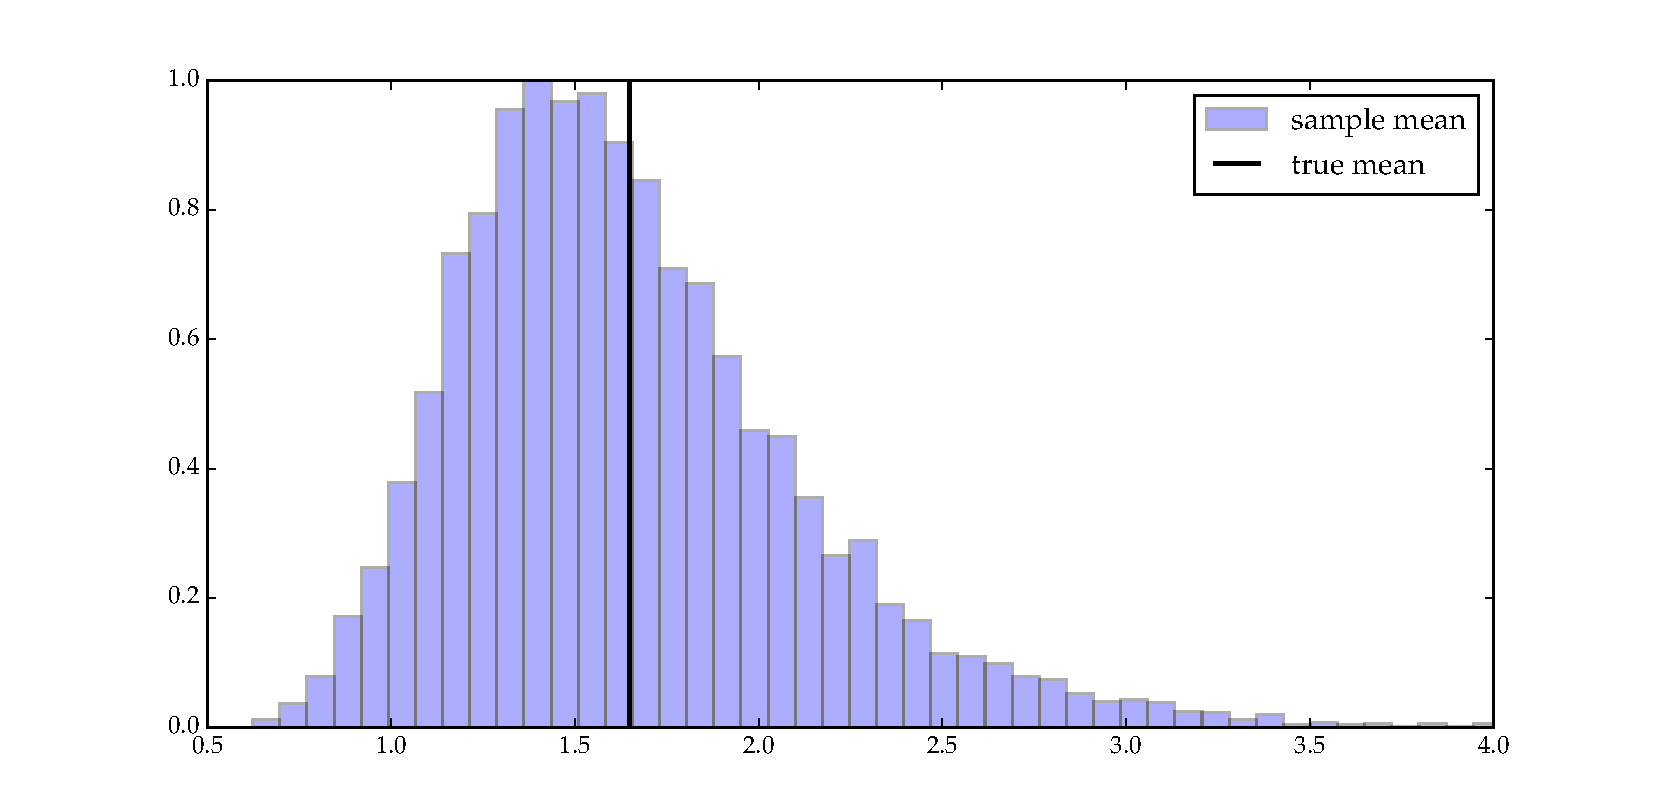
\includegraphics[trim={2em 2em 2em 2em}, clip]{lognorm_sample_mean.pdf}}
    \caption{\label{f:lognorm_sample_mean} Sampling distribution of $\bar x_N$
    when $N=20$ and data are {\sc iid} $\lN(0, 1)$}
    \end{figure}
    
\end{frame}

\begin{frame}[fragile]

        \vspace{1em}
        \begin{pythoncode}
    import numpy as np
    
    N = 20
    num_reps = 10000
    xbar_outcomes = np.empty(num_reps)  # Allocate memory
    
    for i in range(num_reps):
        x = np.exp(np.random.randn(N))
        
        # Generate N iid lognormal RVs
        xbar_outcomes[i] = x.mean()
        \end{pythoncode}

\end{frame}

\begin{frame}\frametitle{Desirable Properties}

    \vspace{2em}
    \begin{quote}
    It is desirable that the sampling distribution of an estimator of $\gamma$
    concentrate most of its probability mass in a small neighbourhood around
    $\gamma$, regardless of the joint distribution $\Pdata$ of the sample
    \end{quote}
      
\end{frame}

\begin{frame}

    \vspace{2em}
    Suppose we are estimating the mean of a distribution from a random sample
    of size $20$:
    \begin{itemize}
        \item each sample drawn from $\lN(0, 1)$
    distribution, the mean of which is about 1.65
    \end{itemize}
    
    \vspace{.7em}
    Consider three estimators of the mean:
    \begin{itemize}
        \item mid-range estimator
        \item maximum likelihood estimator 
        \item sample mean
    \end{itemize}
    
    The last two put more
    probability mass in the region around 1.65 -- outperform
    the mid-range estimator in this setting
    
\end{frame}

\begin{frame}

    \vspace{2em}
    \begin{figure}
        \centering
        \scalebox{.4}{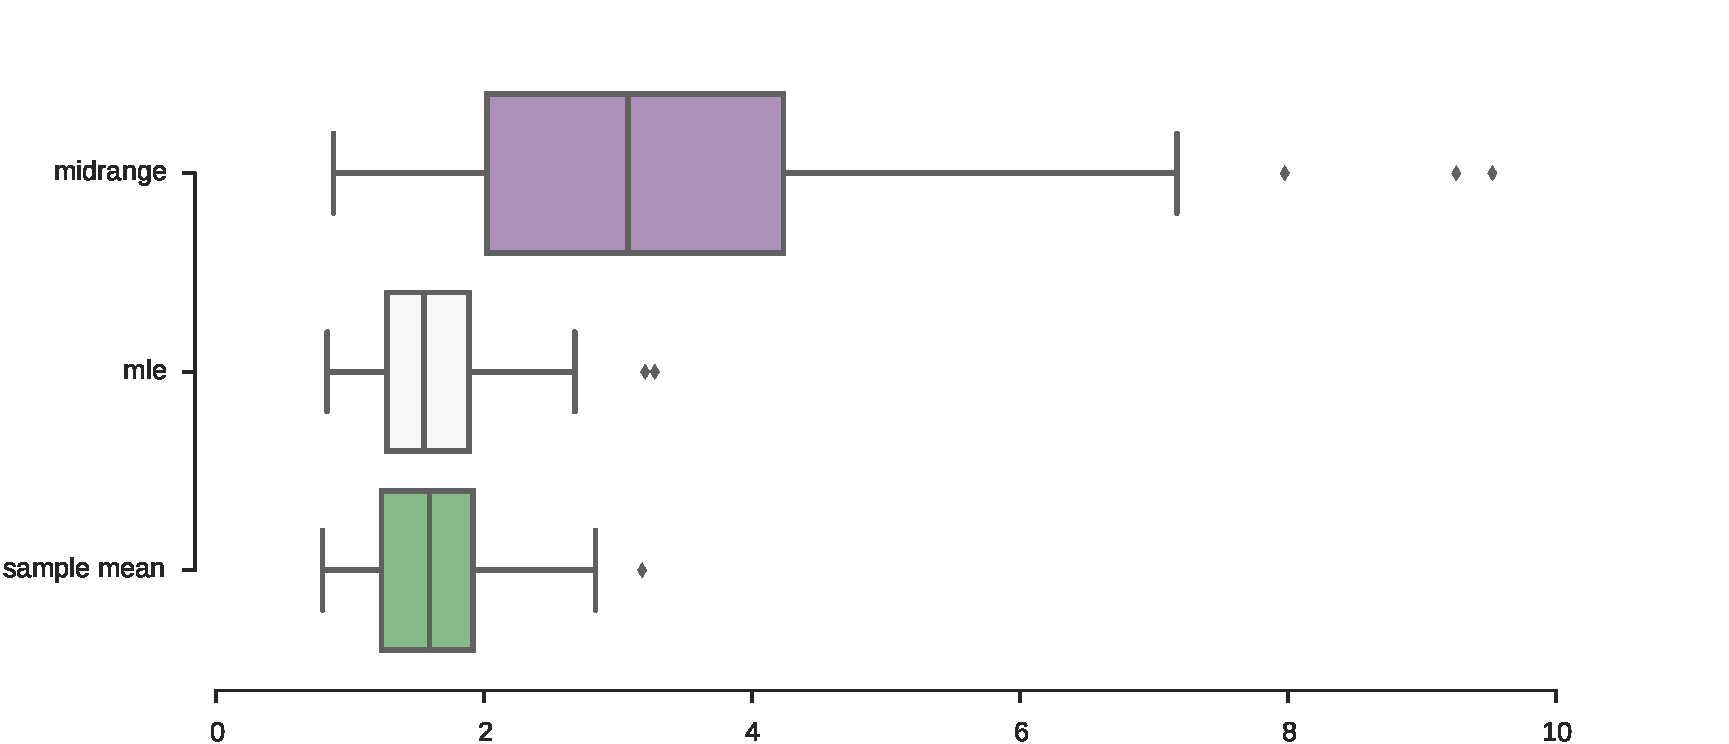
\includegraphics[trim={4em 4em 4em 4em}, clip]{sampling_distributions.pdf}}
        \caption{\label{f:sampling_distributions} Sampling distributions of three estimators of a lognormal mean}
    \end{figure}

\end{frame}

\section{Bootstrap}

\begin{frame}\frametitle{Bootstrap}

    \vspace{2em}
    Sampling
    distributions in reality cannot be observed  because they depend on $\Pdata$
    
    \vspace{.7em}
    For example, suppose $x_1, \ldots, x_N$
    are assumed to be {\sc iid} $\nN(\mu, \sigma^2)$
    with $\mu$ and $\sigma$ unknown
    
    By \eqref{eq:sdsmnc}, the distribution of $\bar x_N$ is $\nN(\mu,
    \sigma^2/N)$ --- we have not pinned down the distribution because
    $\mu$ and $\sigma$ are unknown.

\end{frame}

\begin{frame}

    \vspace{2em}
    In addition:
    \begin{itemize}
        \item  we may not be able to easily write down the sampling
    distribution as a function of the parameters ({\sc iid} lognormals
    in example above)
        \item we
    may not have assumed a parametric form for the distribution of the
    observations
    \end{itemize}
    
\end{frame}


\begin{frame}
    
    \vspace{2em}
    We discuss a general technique to estimate sampling distributions given the data
    
    \vspace{.7em}
    Let $T$ be any statistic and consider its
    sampling distribution:
    %
    \begin{equation*}
        \lL_P(T) 
        := \text{ the distribution of }
        T(x_1, \ldots, x_N) 
    \end{equation*}
    %
    $\text{ when } x_1, \ldots, x_N \iidsim P$
    
    \vspace{.7em}
    Let $x^o_1, \ldots,
    x^o_N$ be a sample of of {\sc iid} draws from $P$
    
    A good estimator of $P$
    given our sample is the empirical distribution $\hat P_N$ generated by $x^o_1,
    \ldots, x^o_N$
    
\end{frame}

\begin{frame}

    \vspace{2em}
    The \navy{bootstrap
    distribution} of $T$:
    %
    \begin{equation*}
        \lL_{\hat P_N}(T) 
        := \text{ the distribution of }
        T(x_1, \ldots, x_N) 
    \end{equation*}
    %
    $\text{ when } x_1, \ldots, x_N \iidsim \hat P_N$
    
    \vspace{.7em}
    The bootstrap distribution is the plug-in estimator of
    the sampling distribution
    
    Is $\lL_{\hat P_N}(T)$ a good approximation to $\lL_P(T)$?
    
    \vspace{.7em}
    Glivenko--Cantelli theorem: $\hat P_N$ will be close to $P$ when $N$ is large
    
    If $Q \mapsto \lL_Q(T)$ is suitably continuous, then 
    $\lL_{\hat P_N}(T)$ will also be close
    to $\lL_P(T)$
    
\end{frame}

\begin{frame}\frametitle{Simulation}

    \vspace{2em}
    To generate draws from $\lL_{\hat P_N}(T)$ on a computer:
    
    
    \vspace{0.4em}
    \begin{algorithmic}[1]
        \State set $\hat P_N = $ the empirical distribution of observed data
        $x^o_1, \ldots, x^o_N$
        \For{$m$ in $1, \ldots, M$}
            \State draw $x_1^b, \ldots, x_N^b$ independently from $\hat P_N$
            \State set $T^b_m = T(x^b_1, \ldots, x_N^b)$
        \EndFor
        \State return the sample $T_1^b, \ldots, T_M^b$ 
    \end{algorithmic}
    \vspace{0.4em}
    
\end{frame}

\begin{frame}

    \vspace{2em}
    Drawing samples from
    $\hat P_N$ easy: make repeated draws from the set $x^o_1, \ldots,
    x^o_N$ with equal probability on each element
    
    \vspace{.7em}
    Julia code to generate draws from $\lL_{\hat P_N}(T)$ 
    -- implement the algorithm as a function returning $M$ bootstrap samples
    
    Arguments to the function:
    \begin{itemize}
        \item \texttt{xo}, the array of observed data
        \item \texttt{stat}, which is a function
    representing $T$
    \end{itemize}
    
\end{frame}

\begin{frame}[fragile]
    
        \vspace{1em}
        \begin{juliacode}
    function bootstrap(xo, stat, M)
        N = length(xo)
        T_b = Array(Float64, M)
        x_b = Array(Float64, N)
        for m in 1:M
            for i in 1:N
                x_b[i] = xo[rand(1:N)]
            end
            T_b[m] = stat(x_b)
        end
        return T_b
    end
        \end{juliacode}

\end{frame}

\begin{frame}[fragile]

    Here's an example function call:
    
    \begin{juliacode}
    julia> bootstrap([1, 2, 3], mean, 3)
    3-element Array{Float64,1}:
    1.66667
    1.0    
    1.66667
    \end{juliacode}
\end{frame}

\begin{frame}[fragile]
    \begin{figure}
    \centering
    \scalebox{.44}{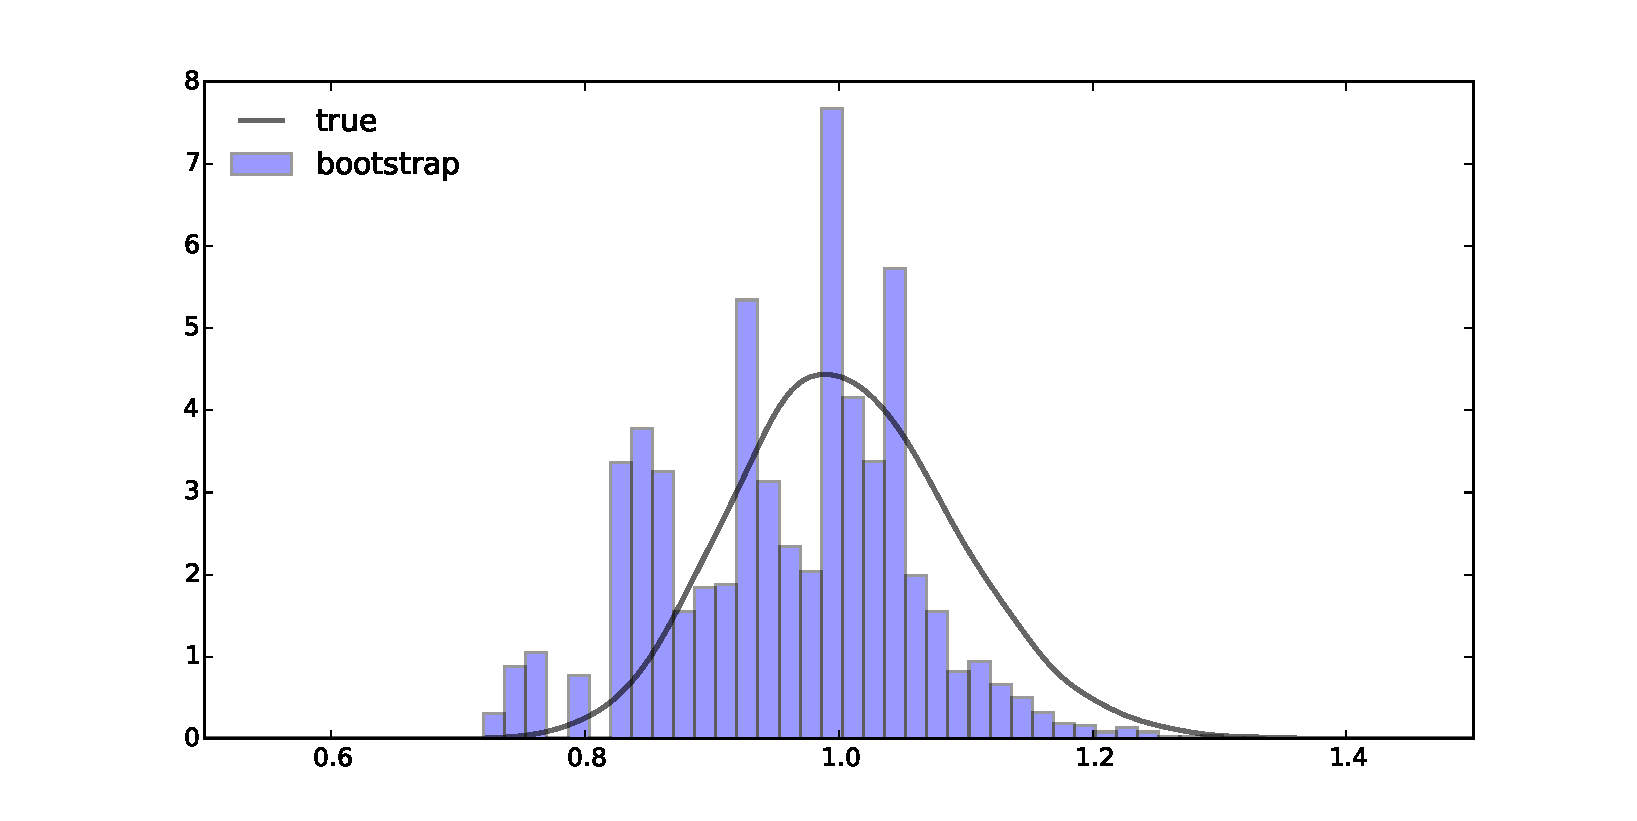
\includegraphics[trim={5em 0em 0em 0em}, 
                    clip]{bootstrap_hist.pdf}}
    \caption{\label{f:bootstrap_hist} Bootstrap draws and 
                    sampling distribution for the median}
    \end{figure}
\end{frame}

\begin{frame}

    \vspace{2em}
    Recall a good estimator is one that concentrates its
    probability mass close to  target feature
    
    How much probability
    mass concentrates usually measured by the variance or standard deviation of
    the sampling distribution

    \vspace{.7em}
    Replace the true standard deviation with an estimate,
    referred to as the \navy{standard error}:
    %
    \begin{equation*}
        \se(\hat \gamma) 
        := \text{ an estimate of the standard deviation of } \hat \gamma
    \end{equation*}
\end{frame}

\begin{frame}

    \vspace{2em}
    \emph{Which} estimate of the standard deviation?
    
    One way to compute a standard error of an
    estimator is to take the sample standard deviation of the bootstrap draws

    \vspace{.7em}
    \Eg
    Next slide shows histogram of draws from the
    bootstrap distribution of the median applied to 2,118 observations of US firm
    sizes by sales
    
    Values are in millions of
    US dollars
    
    The median of the sample itself is 269.9
    
    The sample standard deviation
    of this particular set of bootstrap draws is 25.4

\end{frame}

\begin{frame}

    \begin{figure}
    \centering
    \scalebox{.44}{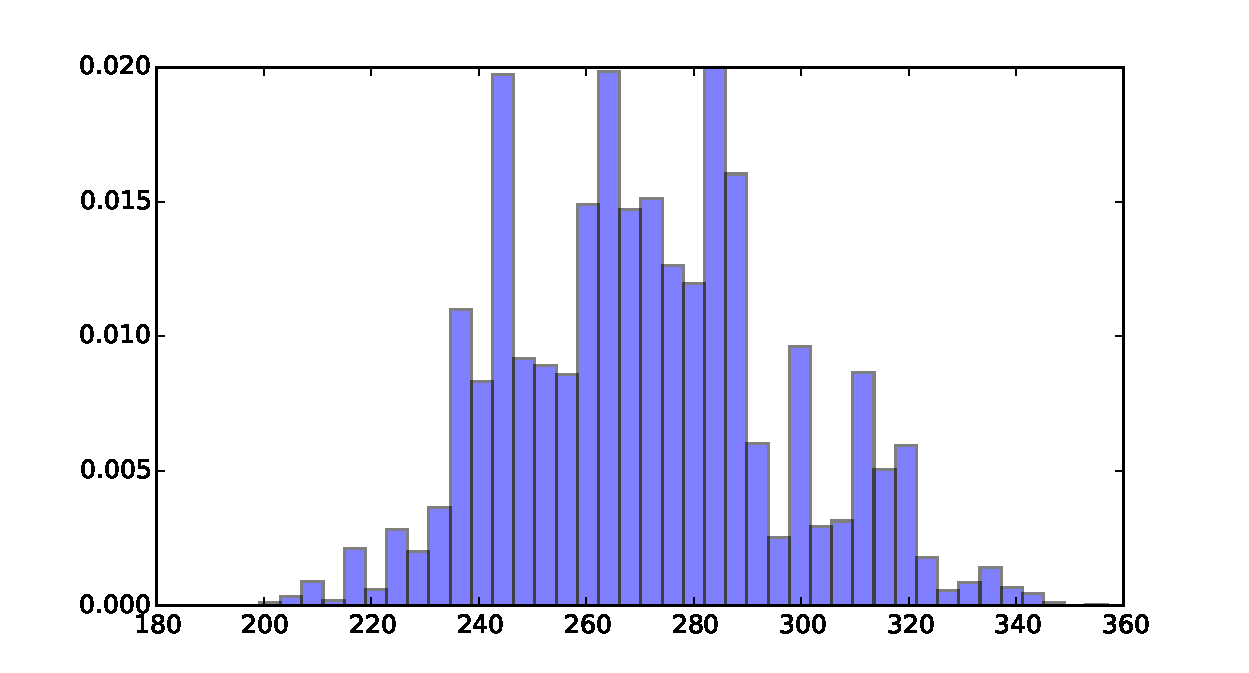
\includegraphics[trim={0em 0em 0em 0em}, clip]{firms_median.pdf}}
    \caption{\label{f:firms_median} Bootstrapped draws for the 
                median of firm sizes by sales}
    \end{figure}

\end{frame}

\section{Evaluating Estimators}

\begin{frame}\frametitle{Evaluating Estimators}

    \vspace{2em}
    Let $\hgamma$ be an estimator of a given feature
    $\gamma = \gamma(P)$.  The \navy{bias} of $\hgamma$ is defined as 
    %
    \begin{equation*}
        \label{eq:bias}
        \text{bias}_P(\hgamma, \gamma) = \EEP  \hgamma - \gamma(P)
    \end{equation*}
    
    \vspace{.7em}
    The estimator $\hgamma$ is called \navy{unbiased} for $\gamma$ over the
    class of distributions $\pP$ if 
    %
    \begin{equation*}
    \text{bias}_P(\hgamma, \gamma) = 0
    \quad \text{for all } P \in \pP
    \end{equation*}
    
\end{frame}

\begin{frame}

    \vspace{2em}
    The notation $\EEP \hgamma$ indicates  expectation is taken under the
    assumption that the data points are {\sc iid} with common distribution $P$
    
    In general, the bias depends on $P$
    
    \vspace{.7em}
    For example, in the {\sc iid} setting,
    the mid-range estimator is
    \begin{itemize}
        \item unbiased estimator of the mean of a uniform distribution 
            on $\RR$ with unknown end points
        \item biased for many other distributions, including the lognormal  
    \end{itemize}
    
\end{frame}

\begin{frame}

    \vspace{2em}
    \Fact\eqref{ET-fa:ubpi}
    Let $P$ be a distribution on $\RR^K$, let $\{\boldx_n\}$
    be a sample with $\lL(\boldx_n) = P$ for all $n$, and let $\hat
    P_N$ be the empirical distribution. If 
    %
    \begin{enumerate}
        \item $\gamma(P) = \int h(\bolds) P(\diff \bolds)$ for some integrable
            function $h$, and
        \item $\hgamma$ is the plug-in estimator $\hgamma = \int h(\bolds)
            \hat P_N(\diff  \bolds) = \frac{1}{N} \sum_{n=1}^N h(\boldx_n)$,
    \end{enumerate}
    %
    then $\hgamma$ is unbiased for $\gamma$ over the set of distributions such
    that $\int h(\bolds) P(\diff \bolds)$ exists
  
\end{frame}

\begin{frame}

    \vspace{2em}
    Proof for fact is immediate from linearity of expectations:
    %
    \begin{multline*}
        \EE \hgamma
        = \EE \left[ \frac{1}{N} \sum_{n=1}^N h(\boldx_n) \right]
        \\ = \frac{1}{N} \sum_{n=1}^N \EE h(\boldx_n) 
        = \int h(\bolds) P(\diff  \bolds) = \gamma(P)
    \end{multline*}
    %
\end{frame}

\begin{frame}
    
    \vspace{2em}
    \Eg
    For any identically distributed sample, the $k$th sample moment is an
    unbiased estimator of the $k$th moment, whenever the latter exists

    \vspace{.7em}
    \Eg
    Let $x_1, \ldots, x_N$ be an {\sc iid} sample with finite variance
    $\sigma^2$
    
    The sample variance $s_N^2$ is, in general, a biased estimator of 
    $\sigma^2$, but not by much
    
    In particular:  
    %
    \begin{equation*}
        \label{eq:esv}
        \EE s^2_N = \sigma^2 \frac{N-1}{N}
    \end{equation*}
    %

\end{frame}

\begin{frame}\frametitle{Variance of Estimators}

    \vspace{2em}
    Sensible estimators almost always have the property that 
    the variance goes to zero as $N \to \infty$
    
    \vspace{.7em}
    \Eg
    If $x_1,\ldots, x_N$ are uncorrelated with common
    finite variance $\sigma^2$, then 
    %
    \begin{equation}
        \label{eq:varsm}
        \var \bar x_N
        = \var \left[ \frac{1}{N} \sum_{n=1}^N x_n \right]
        = \frac{\sigma^2}{N}
    \end{equation}
    %

\end{frame}

\begin{frame}
    
    \vspace{2em}
    \Eg
    Assume the {\sc iid} Gaussian setting of the example above
    
    We showed the sample variance satisfies $\lL(\sigma^{-2} N
    \, s^2_N) = \chi^2(N - 1)$
    
    The variance of a $\chi^2(k)$
    distribution is $2k$
    
    Using this fact and some algebra gives
    %
    \begin{equation*}
        \var  s^2_N  = \frac{2 \sigma^4}{N^2} (N - 1)
    \end{equation*}
    %
\end{frame}

\begin{frame}

    \vspace{2em}
    Is small variance always desirable for an estimator? 
    
    \vspace{.7em}
    If the estimator is
    biased, then perhaps not --- probability mass might be concentrated in the
    wrong place
    
    \vspace{.7em}
    But for an unbiased estimator, low variance
    means probability mass is concentrated around the feature we wish to
    estimate
\end{frame}

\begin{frame}

    \vspace{2em}
    Consider any given estimator -- how do we know whether its
    variance is too low or high? 
    \begin{itemize}
        \item low variance relative
    \end{itemize}
    
    \vspace{.7em}
    One way to approach: take the class of unbiased estimators 
    of a given feature $\gamma$ and find
    the estimator in the class with the lowest variance
    
\end{frame}

\begin{frame}

    \vspace{2em}
    For given $\gamma$
    and given data $\boldx_1,\ldots,\boldx_N$, the estimator in
    the set of unbiased estimators:
    %
    \begin{equation*}
        U_{\gamma} := \{\text{all statistics } \hgamma
            \text{ with } \EE \hgamma = \gamma\}
    \end{equation*}
    %
    that has the lowest variance within this class is called the 
    \navy{minimum variance unbiased estimator}
    
\end{frame}

\begin{frame}

    \vspace{2em}
    However
    
    \begin{itemize}
        \item minimizer may not exist
        \item may be hard to determine in practice
        \item may require strong assumptions on the
    unknown distribution of the data
    \end{itemize}
    
    \vspace{.7em}
    Focus on
    smaller classes than $U_{\gamma}$
    
    For example, the estimator in the set of \emph{linear} unbiased estimators
    %
    \begin{equation*}
        U^{\ell}_{\gamma} := \{\text{all linear statistics } \hgamma 
            \text{ with } \EE \hgamma = \gamma\}
    \end{equation*}
    %
    with the lowest variance---if it exists---is called the \navy{best linear
    unbiased estimator} 
    
\end{frame}

\begin{frame}

    \vspace{2em}
    \Eg
    Let $x_1,\ldots,x_N$ be {\sc iid} with common distribution $P$, where $P$
    has finite mean $\mu \not= 0$ and variance $\sigma^2$
    
    The set of linear
    estimators of $\mu$:
    %
    \begin{align*}
        \bigg\{ 
        \text{all statistics of the form } 
        \hat \mu = \sum_{n=1}^N \alpha_n x_n, \\ \text{ where }
        \alpha_n \in \RR \text{ for } n = 1,\ldots,N
        \bigg\}
    \end{align*}

\end{frame}

\begin{frame}

    \vspace{2em}
    \Eg (cont.)
   The set of linear unbiased estimators of $\mu$:
    %
    \begin{align*}
        U^{\ell}_{\mu} := 
        \bigg\{ 
        \text{all } 
        \hat \mu = \sum_{n=1}^N \alpha_n x_n \text{ with }
        \alpha_n \in \RR,\\ \;\; n = 1,\ldots,N
        \text{ and } 
        \EE \left[ \sum_{n=1}^N \alpha_n x_n \right] = \mu
        \bigg\}
    \end{align*}
    %

\end{frame}

\begin{frame}

    \vspace{2em}
    \Eg (cont.)
    Using linearity of expectations, this set can be rewritten as
    %
    \begin{equation*}
        U^{\ell}_{\mu} := 
        \left\{ 
        \text{all } 
        \hat \mu = \sum_{n=1}^N \alpha_n x_n \text{ with }
        \sum_{n=1}^N \alpha_n = 1
        \right\}
    \end{equation*}
    
    By independence and our rules for variance of sums, 
    the variance of an element of this class is given by
    %
    \begin{equation*}
        \var \left[ \sum_{n=1}^N \alpha_n x_n \right]
        =   \sum_{n=1}^N \alpha_n^2 \var x_n 
        =   \sigma^2 \sum_{n=1}^N \alpha_n^2 
    \end{equation*}
    
    \vspace{.7em}
    To find the best linear unbiased estimator, solve
    %
    \begin{equation*}
        \text{minimize } \; \sigma^2 \sum_{n=1}^N \alpha_n^2 \;
        \text{ over all } \alpha_1,\ldots,\alpha_N \text{ with }
        \sum_{n=1}^N \alpha_n = 1
    \end{equation*}
    
\end{frame}

\begin{frame}

    \vspace{2em}
    \Eg (cont.)
    To solve this constrained optimization problem, we can use the Lagrangian,
    setting
    %
    \begin{equation*}
        L(\alpha_1,\ldots,\alpha_N ; \lambda) := \sigma^2 \sum_{n=1}^N \alpha_n^2 - 
        \lambda \left[\sum_{n=1}^N \alpha_n - 1 \right]
    \end{equation*}
    %
    where $\lambda$ is the Lagrange multiplier
    
    
    Differentiate with respect
    to $\alpha_n$ and set the result equal to zero
\end{frame}

\begin{frame}

    \vspace{2em}
    \Eg (cont.)
    The minimizer $\alpha_n^*$
    satisfies $\alpha_n^* = \lambda  (2 \sigma^2)^{-1}$ for each $n$
    
    In particular, each $\alpha_n^*$ takes the same value, and hence, from the
    constraint $\sum_n \alpha_n^* = 1$, we have $\alpha_n^* = 1/N$
    
    \vspace{.7em}
    Our estimator becomes 
    %
    \begin{equation*}
        \sum_{n=1}^N \alpha_n^* x_n  
        = \bar x_N
    \end{equation*}
    
    
    For {\sc iid} data with finite variance, the sample mean
    is the best linear unbiased estimator of $\mu$

\end{frame}

\begin{frame}

    \vspace{2em}
    However, there's no
    convincing reason to restrict ourselves to unbiased estimators.  In fact, as
    we'll see, there are good reasons not to
    
\end{frame}

\begin{frame}\frametitle{Mean Squared Error}

    \vspace{2em}
    The mean squared error (MSE) of a
    given estimator $\hgamma$ of some feature $\gamma \in \RR^K$:
    %
    \begin{equation}
    \label{eq:mse}
    \mse (\hgamma, \gamma) := \EE \left\{ \, \| \hgamma - \gamma \|^2 \, \right\}
    \end{equation}
    
    \vspace{.7em}
    As with bias, $\mse(\hgamma, \gamma)$ depends on the joint distribution of the data as
    well as the specification of $\hgamma$
    
\end{frame}

\begin{frame}

    \vspace{2em}
    Mean squared error takes into account both bias and variance; the scalar case:
    %
    \begin{equation}
        \label{eq:dmse}
        \mse (\hgamma, \gamma) = \var \hgamma + \text{bias}(\hgamma, \gamma)^2
    \end{equation}
    
    \vspace{.7em}
    \Eg
    Consider an {\sc iid} sample $x_1, \ldots,
    x_N$ with common distribution $\nN(\mu, \sigma^2)$

    Consider the sample variance $s_N^2$
    
    We showed (example~\ref{ET-eg:sdq2} in ET) $\var  s^2_N
    = 2 \sigma^4 N^{-2} (N - 1)$
    
    Combine this result with
    \eqref{eq:dmse} and $\EE s^2_N = \sigma^2 \frac{N-1}{N}$ to arrive at
    %
    \begin{equation*}
        \mse \left( s^2_N, \sigma^2 \right) 
        = \frac{2 \sigma^4}{N^2} (N - 1) 
        + \left[ \sigma^2 \frac{N-1}{N} - \sigma^2 \right]^2
        = \frac{\sigma^4}{N^2}  (2N - 1) 
    \end{equation*}
    
\end{frame}

\begin{frame}

    \vspace{2em}
    Typically there is a trade-off between bias and variance to minimise MSE:
    \begin{itemize}
        \item lower variance costs more bias and vice-versa
        \item interior solutions: we can often reduce variance significantly by
        accepting a small amount of bias
    \end{itemize}

\end{frame}

\begin{frame}

    \vspace{2em}
    \Eg
    Let $\hgamma$ be any unbiased estimator of a feature $\gamma \in \RR$
    
    Let $v := \var \hgamma$
    
    Consider the class of estimators $\setntn{ \lambda \hgamma
    }{\lambda \in \RR}$
    
    \vspace{.7em}
    Value of $\lambda$ that minimizes $\mse(\lambda \hgamma, \gamma)$ is
    %
    \begin{equation}
        \label{eq:oeib}
        \lambda^* := \frac{\gamma^2}{\gamma^2 + v}
    \end{equation}
    %
    (exercise~\ref{ET-ex:udmmse})
    
    Unbiased estimator does not minimize MSE unless $v = 0$

\end{frame}

\begin{frame}

    \vspace{2em}
    For most sensible estimators, $v$ converges to zero as the sample size $\to
    \infty$
    
    Unbiased estimators only approach optimality
    when the data size is large
    
    \vspace{.7em}
    Here ``large" should be understood as relative
    to model complexity
    
    More complex models need more data to be estimated
    effectively
    
\end{frame}

\begin{frame}\frametitle{Stein's Example}

    \vspace{2em}
    Consider a population of
    $K$ individuals, where the $k$th individual has idiosyncratic ability
    $\mu_k \in [0, 1]$
    
    For each agent, we observe $N$ noisy signals of
    ability, each of the form $x_{kn} = \mu_k + \epsilon_{kn}$, $n=1, \ldots, N$
    
    The noise terms $\epsilon_{kn}$ are all independent $\nN(0, \sigma^2)$
   
   \vspace{.7em}
    Objective: estimate the parameter vector $\boldmu = (\mu_1, \ldots, \mu_K)$ 
    given the data from the observations $x_{nk}$
    
    Assume
    only $\boldmu$ is unknown
    
\end{frame}

\begin{frame}

    \vspace{2em}
    Vector sample mean
    %
    \begin{equation*}
    \bar \boldx_N 
    =
    \begin{pmatrix}
        \frac{1}{N} \sum_{n=1}^N x_{1n}
        \\
        \vdots
        \\
        \frac{1}{N} \sum_{n=1}^N x_{Kn}
    \end{pmatrix}
    \end{equation*}
    
    maximum likelihood estimator of ability, and best
    linear unbiased

\end{frame}

\begin{frame}

    \vspace{2em}
    However, when $K > 2$,  there exists an alternative estimator
    $\hboldmu_N$ such that
    %
    \begin{equation}
        \label{eq:mlii}
        \EE \left\{ \, \| \hboldmu_N - \boldmu \|^2 \,  \right\}
        < \EE \left\{ \, \| \bar \boldx_N - \boldmu \|^2 \,  \right\}
        \quad
        \text{for all } \boldmu \in \RR^K
    \end{equation}
    
    Estimator $\hboldmu_N$ uniformly dominates $\bar \boldx_N$ in terms of
    MSE, for all possible values of $\boldmu$!  
    
    \vspace{.7em}
    The estimator in question is what
    is now known as the \navy{James--Stein estimator}:
    %
    \begin{equation*}
        \hboldmu_N 
        = \kappa \,
        \bar \boldx_N
        \quad \text{where} \quad
        \kappa :=
            1 - \frac{K - 2 }{N} \frac{\sigma^2}{ \| \bar \boldx_N \|^2}
    \end{equation*}
    
\end{frame}


\begin{frame}

    \vspace{2em}
    Intuition from simulation:
    \begin{itemize}
        \item set $K=200$, $N=5$ and
    $\sigma=1$
        \item 5 noisy observations on the ability of each of 200 agents
        \item for each agent, choose ability $\mu_k$ independently 
                from a uniform distribution on $[0, 1]$
        \item compute the estimators $\bar
    \boldx_N$ and $\hboldmu_N$ and the corresponding error vectors
    
    See \url{johnstachurski.net/emet} for code

    \end{itemize}
    
\end{frame}

\begin{frame}

    \begin{figure}
    \centering
    \scalebox{.4}{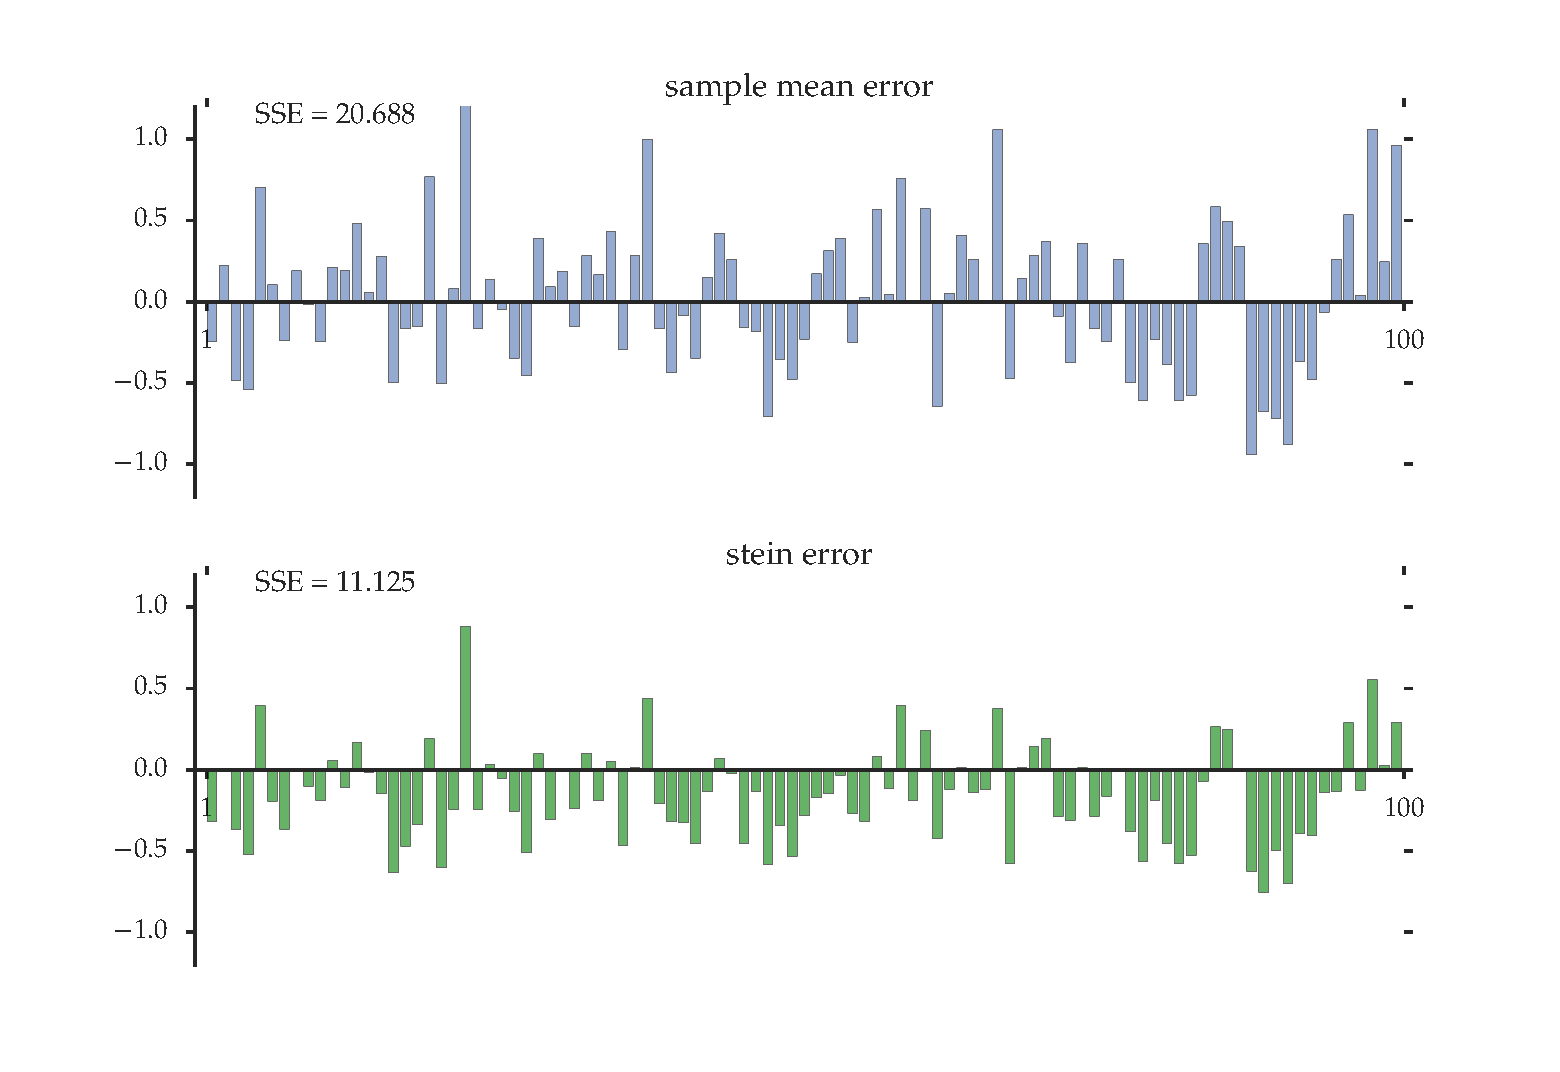
\includegraphics[trim={2em 2em 2em 2em}, clip]{stein.pdf}}
    \caption{\label{f:stein} Error vectors for the two estimators }
    \end{figure}
    
\end{frame}

\begin{frame}

    \vspace{2em}
    Errors for the James-Stein estimator are downward biased 
    and also smaller than the errors of the sample mean estimator
    
    \vspace{.7em}
    The squared
    norm of the error vectors for the sample me is nearly
    twice as large

\end{frame}

\section{Asymptotic Properties}

\begin{frame}\frametitle{Asymptotic Properties}

    \vspace{2em}
    Asymptotic theory
    \begin{itemize}
        \item concerns whether or not the sampling distribution of 
            an estimator increasingly concentrates around the feature we wish to estimate
        \item the rate at which an estimator ``concentrates" or converges 
        \item the shape of the sampling distribution in large samples
    \end{itemize}
    

\end{frame}

\begin{frame}

    \vspace{2em}
    Let $\{\hgamma_N\}$ be a sequence of estimators of a given feature
    $\gamma$, based on a sample of size $N$
    
    \vspace{.7em}
    We say $\hgamma_N$ is
    \navy{consistent} for $\gamma$ if:
    %
    \begin{equation}
        \label{eq:consistent}
        \hgamma_N \toprob \gamma
        \quad \text{as} \quad 
        N \to \infty
    \end{equation}
    
    The definition is the same whether the estimators are vector
    or scalar-valued
    
    The statement that $\hgamma_N$ is consistent means
    sequence $\{\hgamma_N\}$ is consistent
\end{frame}

\begin{frame}

    \vspace{2em}
    As for bias, whether consistency holds depends not just on $\hat
    \gamma_N$ but also on the joint
    distribution of the data
    
    \vspace{.7em}
    If we say that $\hgamma_N$ is consistent over a class
    of distributions $\pP$, we mean:
    
    \begin{equation*}
        \hgamma_N \toprob \gamma
        \quad \text{as} \quad 
        N \to \infty
    \end{equation*}
    
    Holds true for any distribution in $\pP$
    
\end{frame}

\begin{frame}

    \vspace{2em}
    \Eg
    The sample mean $\bar x_N$ of any {\sc iid} sample is consistent for the
    mean over the class of distributions on $\RR$
    with finite first moment
    
    Indeed, if $P$ is such a distribution and $x_1,
    \ldots, x_N$ are {\sc iid} draws from $P$, then the law of large numbers gives
    %
    \begin{equation*}
        \frac{1}{N} \sum_{n=1}^N x_n \toprob \int s P(\diff s)
         \quad \text{ as } \quad N \to \infty
    \end{equation*}
    
\end{frame}

\begin{frame}

    \vspace{2em}
    More generally,  $\hgamma_N = \frac{1}{N}
    \sum_{n=1}^N h(\boldx_n)$ is consistent for $\gamma = \int h(\bolds) P(\diff \bolds)$
    whenever
    %
    \begin{enumerate}
        \item $\boldx_1, \ldots, \boldx_N$ is an {\sc iid} sample with
            $\lL(\boldx_n) = P$ for all $n$ and
        \item $\int h(\bolds) P(\diff \bolds)$ exists.
    \end{enumerate}
    
    \vspace{.7em}
    For example, the $k$th sample moment is consistent for the $k$th moment over
    the class of distributions with finite $k$th moment
    
\end{frame}

\begin{frame}

    \Eg
    For any {\sc iid} sample $x_1, \ldots, x_N$ with finite variance, the
    sample variance $s^2_N$ is consistent for the variance
    
    Can be
    established from:
    %
    \begin{equation}
        \label{eq:sn2e}
        s_N^2 = \frac{1}{N} \sum_{n=1}^N (x_n - \mu)^2 - (\bar x_N - \mu)^2
    \end{equation}
    %
    where $\mu$ is the common mean (see ex.~\ref{ET-ex:sn2e} and its
    solution)
    
    \vspace{.7em}
    Applying the law of large numbers to \eqref{ET-eq:sn2e}, the
    first term converges to $\sigma^2$,  while $(\bar x_N - \mu)
    \toprob 0$, and hence $(\bar x_N - \mu)^2 \toprob 0$ by 
    fact~\ref{ET-fa:reconpro} on page~\pageref{ET-fa:reconpro} in ET
    
    Consistency of $s^2_N$ follows

\end{frame}

\begin{frame}

    \vspace{2em}
    \Fact\eqref{ET-fa:cpc}
    If $\hgamma_N$ is consistent for $\gamma$ and $g$ is any continuous
    function, then $g(\hgamma_N)$ is consistent for $g(\gamma)$

    \vspace{.7em}
    \Eg
    The sample standard deviation $s_N = \sqrt{s^2_N}$ is consistent for the
    standard deviation whenever $s^2_N$ is consistent for the variance
    
\end{frame}

\begin{frame}\frametitle{Asymptotic Distributions}

    \vspace{2em}
    Central limit theorem tells us
    (remarkably!) the sample mean is always asymptotically Gaussian, provided
    that the underlying observations have finite second moment
    
    Let $\{\hgamma_N\}$ be a sequence of estimators 
    for some feature $\gamma$
    
    \vspace{.7em}
    We say that $\hgamma_N$ is
    \navy{asymptotically normal} if
    there exists a positive definite matrix $\Sigma$ such that
    %
    \begin{equation}
        \label{eq:asn}
        \sqrt{N} (\hgamma_N - \gamma) \tod \nN(\boldzero, \Sigma)  
        \quad \text{as} \quad
        N \to \infty
    \end{equation}
    %
    When \eqref{eq:asn} holds, $\Sigma$ is called the \navy{asymptotic
    variance--covariance matrix} of $\hgamma_N$
    
\end{frame}

\begin{frame}

    \Eg Let $x_1, \ldots, x_N$ be {\sc iid} with common 
    mean $\mu$ and variance $\sigma^2$
    
    If $\EE[x_n^4] < \infty$,
    then the sample variance $s_N^2$ is asymptotically normal
    with 
    %
    \begin{equation}
        \label{eq:avarsn2}
        \sqrt{N}(s_N^2 - \sigma^2)
        \tod \nN(0, m_4 - \sigma^4)
        \quad 
    \end{equation}
    
    $\text{where} \quad
        m_4 := \EE[(x_n - \mu)^4]$
    
    \vspace{.7em}
    To show this, recall 
    %
    \begin{equation}
        s_N^2 = \frac{1}{N} \sum_{n=1}^N (x_n - \mu)^2 - (\bar x_N - \mu)^2
    \end{equation}
        
\end{frame}

\begin{frame}
    
    \vspace{2em}
    \Eg (cont.) 
    We can modify this expression to get
    %
    \begin{multline}
        \label{eq:sn2es}
        \sqrt{N}(s_N^2 - \sigma^2)
        \\ = \sqrt{N} 
        \left[ 
            \frac{1}{N} \sum_{n=1}^N (x_n - \mu)^2 - \sigma^2
        \right]
        -  \sqrt{N} (\bar x_N - \mu)^2 
    \end{multline}
    
    \vspace{.7em}
    The last term on the right-hand side of \eqref{eq:sn2es} 
    converges to zero in probability:
    %
    \begin{equation*}
        \sqrt{N} (\bar x_N - \mu)^2
        = a_N b_N
        \quad 
    \end{equation*}
    %
    $\text{where} \quad
        a_N := \sqrt{N} (\bar x_N - \mu), \;
        b_N := \bar x_N - \mu$
        
\end{frame}

\begin{frame}

    \vspace{2em}
    \Eg (cont.) By the CLT, the LLN and fact~\ref{ET-fa:sluti}
    on page~\pageref{ET-fa:sluti} of ET, we
    have $a_N b_N \toprob 0$

    \vspace{.7em}
    To complete the proof, let $Y_n := (x_n - \mu)^2$
    
    The first term in \eqref{eq:sn2es} can then be written as
    $\sqrt{N}(\bar Y_N - \EE [Y_n])$
    
    Apply the CLT, then the expression converges to
    a zero-mean normal with variance 
    %
    \begin{equation*}
        \var Y_n
        = \EE[ (Y_n - \sigma^2)^2 ]
        = \EE[ (x_n - \mu)^4 - 2(x_n - \mu)^2 \sigma^2 + \sigma^4 ]
    \end{equation*}
    
    The claim follows
    
\end{frame}

\begin{frame}
    
    \vspace{2em}
    \Eg Under the same assumptions as the example above, the sample standard
    deviation is also asymptotically normal, with 
    %
    \begin{equation}
        \label{eq:avarsn}
        \sqrt{N}(s_N - \sigma)
        \tod \nN\left(0, \frac{m_4 - \sigma^4}{4 \sigma^2} \right)
    \end{equation}
    %
    See exercise~\ref{ET-ex:ssdcan} for a proof
    
    \vspace{.7em}
    \Eg
    Asymptotic normality implies consistency.  In particular, if
    $\{\hgamma_N\}$ satisfies 
    %
    $$ \sqrt{N} (\hgamma_N - \gamma) \tod \nN(\boldzero, \Sigma)  
        \quad \text{as} \quad
        N \to \infty$$
    %
    then $\hgamma_N \toprob \gamma$
    as $N \to \infty$ (see ex.~\ref{ET-ex:anormic})

\end{frame}

\begin{frame}

    \vspace{2em}
    Asymptotic normality implies a rate at which 
    $\hgamma_N$ converges to $\gamma$
    
    \vspace{.7em}
    If $\hgamma_N$ is asymptotically
    normal, then $\sqrt{N} ( \hgamma_N - \gamma)$ does not diverge
    \begin{itemize}
    \item $\hgamma_N - \gamma$ goes to zero
    fast enough to offset the diverging term $\sqrt{N}$
    \end{itemize}
    
    \vspace{.7em}
    We say that an asymptotically normal estimator $\hgamma_N$
    is \navy{$\sqrt{N}$-consistent} for $\gamma$
    
\end{frame}

\begin{frame}

    \vspace{2em}
    Important! Asymptotic normality gives us an
    approximation to the entire sampling distribution 
    ---  means of performing inference
    
    To be discussed in Ch. 10.
    
\end{frame}

\section{Decision Theory}

\begin{frame}\frametitle{Decision Theory}

    \vspace{2em}
    We still lack convincing general theory of optimality of
    estimators that rests on objective criteria
    
    \vspace{.7em}
    For example, consider the theory of minimum variance
    unbiased estimators:
    \begin{itemize}
        \item initially seems attractive because it can potentially
            yield estimators without any subjective judgment on the part of the
            statistician
        \item there are simple settings where minimum variance unbiased
    estimators are \emph{inadmissible} -- we discuss below
    
    \end{itemize}

\end{frame}

\begin{frame}

    \vspace{2em}
    Without a fully objective theory of ``good" estimators,  
    we are forced to take a stand on our
    criteria for assessing estimators in different situations
    
    \vspace{.7em}
    The estimation problem is not fully specified until we make our
    preferences explicit
    
    \begin{itemize}
        \item specify preference in terms of loss 
        \item full description of an estimation problem
            includes specification of the loss incurred when an estimator performs
            poorly
    \end{itemize}
    
\end{frame}

\begin{frame}

    \vspace{2em}
    Let's frame these ideas in line with the seminal work of 
    \cite{wald1939contributions} and subsequent research on decision theory
    
    \vspace{.7em}
    A general decision problem consists of
    %
    \begin{enumerate}
        \item a sample space $\xX$,
        \item an action space $\aA$,
        \item a set $\ddD$ of decision rules, which are maps $d \colon \xX \to \aA$
        \item a universe $\Theta$ of possible states of the world, with typical
            element $\theta$,
        \item a set of probability distributions $\{P_\theta\}$ over the sample
            space $\xX$, and
        \item a loss function $L \colon \aA \times \Theta \to \RR$
            %
    \end{enumerate}
\end{frame}

\begin{frame}

    \vspace{2em}
    The loss function has the following interpretation:
    %
    \begin{align*}
        L(a, \theta) =  \text{loss from choosing action $a$ when state of world is} \,\theta
    \end{align*}
    
    \vspace{.7em}
    The state of the world treated as unknown
    
    The problem is to
    choose a decision rule $d \in \ddD$ generating ``low loss"
    
\end{frame}

\begin{frame}

    \vspace{2em}
    Define \navy{risk}:
    %
    \begin{equation*}
        \label{eq:waldrisk}
        \risk(d, \theta) := \int L[d(x), \theta ] \, P_\theta(\diff x)
    \end{equation*}
    %
    The integral is over all $x \in \xX$
    
     \vspace{.7em}
    The notation $\risk$ is used to
    distinguish this decision-theoretic concept of risk from $R(f)$, the
    prediction risk of policy $f$ as we defined in Equation \eqref{ET-eq:rf} in ET
    
\end{frame}


\begin{frame}

    \vspace{2em}
    \Eg (Knightian uncertainty)
    Let $\pi$ be an inflation rate and let 
    $x$ be a noisy signal of inflation received by firms
    
    Each firm responds
    by choosing a price $p = p(x)$ for their product
    
    $\Pi(p,
    \pi)$ represents profits from choosing price $p$ when the inflation
    rate is $\pi$ -- let loss be negative profits
    
    Risk:
    %
    \begin{equation*}
        \risk(p, \theta) 
        = - \int \Pi(p(x), \pi) P_\theta(\diff x, \diff \pi)
    \end{equation*}
    
    \vspace{.7em}
    If the distribution $P_\theta$ is known to the firm (think of
    $\{P_\theta\}$ as a singleton), then we have a standard problem of
    choosing price to maximize expected profits under known probabilities for
    outcomes
    
    If, however, $P_\theta$ is not known, we have a problem of
    \navy{Knightian uncertainty}

\end{frame}

\begin{frame}

    \vspace{2em}
    Problem of choosing estimators a special case of the decision theory
    described above
    
    \vspace{.7em}
    Suppose we observe data $\zdata$ taking values in
    $\Zdata$ with joint distribution $P_\theta$ indexed by $\theta \in \Theta$
    (The set $\Theta$ can be infinite dimensional.)
    
    We wish to estimate some $S$-valued feature $\gamma_\theta = \gamma(P_\theta)$
    using this data
    
\end{frame}

\begin{frame}

    \vspace{2em}
    An estimator in this context is a decision rule $\hat
    \gamma$ mapping $\Zdata$ to the action space $\aA = S$
    
    \vspace{.7em}
    If we specify the
    loss $L(\hat \gamma, \theta)$ of choosing $\hat \gamma$ when the state of the
    world is $\theta$, our risk becomes
    %
    \begin{equation*}
        \label{eq:norage}
        \risk(\hat \gamma, \theta) 
        = \int_{\Zdata} L(\hat \gamma(\boldz), \gamma_\theta) P_\theta(\diff \boldz)
    \end{equation*}

\end{frame}

\begin{frame}

    \Eg
    Suppose we want to estimate expected returns $\mu_\theta :=
    \int s P_\theta(\diff s)$ to holding an asset based on {\sc iid}
    observations $x_1, \ldots, x_N$ from $P_\theta$
    
    \vspace{.7em}
    With quadratic loss for
    prediction error and the sample mean as our estimator, the risk is
    %
    \begin{equation*}
        \label{eq:rsmean}
        \risk(\bar x_N, \theta) 
        = \EE_\theta \left[  (\bar x_N - \mu_\theta)^2 \right]
    \end{equation*}
    
    Since $\bar x_N$ is unbiased for $\mu_\theta$, this evaluates to the
    variance of $\bar x_N$ under $P_\theta$, which is
    equal to $\sigma_\theta^2/N = \int (s - \mu_\theta)^2 P_\theta (\diff s)/N$ 
    
\end{frame}

\begin{frame}

    \vspace{2em}
    In the preceding example, the risk of the estimator is its MSE
    
    But no reason to confine ourselves to quadratic
    loss:
    
    \vspace{.7em}
    \Eg
    Common to use the sample median rather the sample mean as 
    an estimate of central tendency of housing prices at a location
    
    Large upper tails distort the price faced by a ``typical buyer"
    
    Choice of median over mean can be understood as 
    minimization of a different loss function when estimating price given
    pricing data
    
\end{frame}

\begin{frame}\frametitle{Choosing Decision Rules}

     \vspace{2em}
    Natural idea for making optimal decisions and for
    choosing optimal estimators: choose decision rules with
    low risk
    
    \vspace{.7em}
    However, risk depends on the unknown state of the world $\theta$
    \begin{itemize}
        \item risk-minimizing
    decision rule also depends on the unknown value $\theta$
    \end{itemize}

    Knightian uncertainty -- we can't evaluate risk because
    we don't know the probabilities

\end{frame}

\begin{frame}

    \vspace{2em}
    \Eg
    Consider again expected returns $\mu_\theta :=
    \int s P_\theta(\diff s)$ to holding an asset based on {\sc iid}
    observations $x_1, \ldots, x_N$ from $P_\theta$
    
    The risk of the
    sample mean is equal to $\sigma_\theta^2/N$ for every value
    of $\theta$
    
    Consider now a new estimator $\hgamma$ that is identically
    equal to $1$:  predicting 100\% return on our
    investment
    
    Great estimator when true mean returns are $1$:
    %
    \begin{equation*}
        \mu_\theta = 1
        \quad \implies \quad
        \risk(\hgamma, \theta) 
        = \EE \left[  (1 - \mu_\theta)^2 \right] 
        =   (1 - 1)^2  
        = 0
    \end{equation*}
    
    We have $\risk(\hgamma, \theta) <
    \risk(\bar x_N, \theta)$ whenever $\sigma_\theta > 0$
    
\end{frame}

\begin{frame}
    \vspace{2em}
    But
    if $\mu_\theta$ diverges sufficiently from $1$, then
    %
    \begin{equation*}
        \risk(\hgamma, \theta) 
        =   (1 - \mu_\theta)^2
        >  \frac{\sigma_\theta^2}{N} 
        = \risk(\bar x_N, \theta)
    \end{equation*}
    %
\end{frame}

\begin{frame}\frametitle{Inadmissibility}

    \vspace{2em}
    We cannot, in general, choose estimators
    based on lowest risk in a classical setting
    
    We can exclude estimators always dominated in terms of risk --- inadmissible estimators
    
    \vspace{.7em}
    A decision
    rule $d$ is called \navy{inadmissible} if
    there exists a second rule $e$ such that 
    %
    \begin{enumerate}
        \item $\risk(e, \theta) \leq \risk(d, \theta)$ for all $\theta \in
            \Theta$ and
        \item $\risk(e, \theta) < \risk(d, \theta)$ for at least one $\theta \in
            \Theta$
    \end{enumerate}
    
    A decision rule that is not inadmissible is called \navy{admissible}
    
\end{frame}

\begin{frame}

    \vspace{2em}
    \Eg
    Consider again estimating the mean when $L$ is quadratic and the
    universe of distributions is the multivariate Gaussians
    
    Vector sample mean
    %
    \begin{equation*}
    \bar \boldx_N 
    =
    \begin{pmatrix}
        \frac{1}{N} \sum_{n=1}^N x_{1n}
        \\
        \vdots
        \\
        \frac{1}{N} \sum_{n=1}^N x_{Kn}
    \end{pmatrix}
    \end{equation*}
    
    Recall that when $K > 2$,  there exists estimator
    $\hboldmu_N$ such that
    %
    \begin{equation}
        \EE \left\{ \, \| \hboldmu_N - \boldmu \|^2 \,  \right\}
        < \EE \left\{ \, \| \bar \boldx_N - \boldmu \|^2 \,  \right\}
        \quad
        \text{for all } \boldmu \in \RR^K
    \end{equation}
    
    Thus, in this case, the vector sample mean is inadmissible as an estimator of the mean
    
\end{frame}

\begin{frame}\frametitle{Minimax Rule}
    
    \vspace{2em}
    A decision rule $d_m$ is called a \navy{minimax} rule if
    %
    \begin{equation*}
        r(d_m) \leq r(d) 
        \text{ for all } d \in \ddD
        \quad \text{where} \quad
        r(d) := \sup_{\theta \in \Theta} \risk(d, \theta)
    \end{equation*}
    
    \vspace{.7em}
    Minimax rule performs well in the worst possible state of the
    world
 
\end{frame}

\begin{frame}\frametitle{Bayes Rules and Bayes Risk}

    \vspace{2em}
    Consider now a prior distribution $\pi = \pi(\theta)$ over states of the world
    
    In addition each $P_\theta$ is now restricted to be a density $p(x \given
    \theta)$
    
    \vspace{.7em}
    As in \S\ref{ET-ss:be}, we obtain the posterior for $\theta$ from the prior
    given data $x$ via Bayes' law:
    %
    \begin{equation*}
        \pi(\theta \given x) 
        = \frac{p(x \given \theta) \pi(\theta)} {p(x)}
        \qquad 
        (x \in \xX, \; \theta \in \Theta)
    \end{equation*}
    
\end{frame}

\begin{frame}

    \vspace{2em}
    Given decision rule $d$ with risk function $\risk(d, \theta)$, 
    the \navy{posterior risk} or \navy{Bayes risk} of $d$ is 
    %
    \begin{equation*}
        r_\pi(d) := \int \risk(d, \theta) \pi(\theta) \diff \theta
    \end{equation*}
    
    \vspace{.7em}
    A decision rule $d$ that minimizes the Bayes risk is called a \navy{Bayes
    rule}
    
    If $d$ is an estimator, then a Bayes rule is called a \navy{Bayes
    estimator}
    
\end{frame}

\begin{frame}

    \vspace{2em}
    Attractive features of Bayes rules, and Bayes
    estimators in particular:
    
    \begin{itemize}
        \item Bayes rules are always admissible under
                mild regularity conditions
        \item Bayes rules can be computed
                as a function of observed data, meaning that we don't have to concern
                ourselves with how to act in situations that potentially never occur
    \end{itemize}
    
\end{frame}

\begin{frame}

    \vspace{2em}
    To understand the second point, write the joint density of
    $(x, \theta)$ as either $p(x \given \theta) \pi(\theta)$ or 
    $\pi(\theta \given x) p(x)$
    
    Use a change in order of integration followed by this identity,
    the Bayes risk becomes:
    %
    \begin{align*}
        r_\pi(d) 
        & = \int_\Theta 
            \left\{
                \int_\xX
                L(d(x), \theta) p(x \given \theta)
                \diff x
            \right\}
            \pi(\theta) 
            \diff \theta   
        \\
        & = \int_\xX 
            \left\{
                \int_\Theta
                L(d(x), \theta) p(x \given \theta) \pi(\theta) 
                \diff \theta   
            \right\}
                \diff x
        \\
        & = \int_\xX 
            \left\{
                \int_\Theta
                L(d(x), \theta) \pi(\theta \given x) 
                \diff \theta   
            \right\}
                p(x)
                \diff x
    \end{align*}
    
\end{frame}

\begin{frame}

    \vspace{2em}
    It follows from this last expression that $d$ will be a Bayes rule whenever 
    %
    \begin{equation}
        \label{eq:bmv}
        d(x) \in \argmin_{a \in \aA} 
                \int_\Theta
                L(a, \theta) \pi(\theta \given x) 
                \diff \theta   
                \quad \text{for all $x \in \xX$}
    \end{equation}
    
    \vspace{.7em}
    Akin to the scenario encountered in dynamic
    programming after applying Bellman's principle of optimality:  once we know
    the value function, we can choose the optimal action just by responding to any 
    observed state
\end{frame}

\begin{frame}
     
    \vspace{2em}
    \Eg
    Let $\theta$ be scalar, let $L(a, \theta) = (a - \theta)^2$ and let
    $\pi(\theta \given x)$ be the posterior distribution of $\theta$ given
    data $x$.  The Bayes estimator of $\theta$ is, by \eqref{eq:bmv} above, the
    solution to 
    %
    \begin{equation*}
           \min_{a \in \RR} 
            \int (a - \theta)^2 \pi(\theta \given x) \diff \theta   
    \end{equation*}
    
    \vspace{.7em}
    The minimizer is the mean of 
    $\pi(\theta \given x)$ (exercise~\ref{ET-ex:minqrisk} on
    page~\pageref{ET-ex:minqrisk})
    
    \vspace{.7em}
    With quadratic loss, the Bayes
    estimator is the mean of the posterior distribution
    
\end{frame}

\begin{frame}

    \vspace{2em}
    \Eg
    If we repeat the setting of above but with the absolute
    loss function $L(a, \theta) = |a - \theta|$ instead of quadratic loss, the 
    Bayes estimator of $\theta$ is
    %
    \begin{equation*}
           \argmin_{a \in \RR} 
            \int |a - \theta| \pi(\theta \given x) \diff \theta   
    \end{equation*}
    %
    $\pi(\theta \given x)$ (exercise \ref{ET-ex:mmed2})

\end{frame}

\end{document}
